%%
%% This is file `main.tex' based on `sample-sigconf.tex' (q.v. for spurce of that,
%%
%% IMPORTANT NOTICE:
%% 
%% For the copyright see the original source file `sample-sigconf.tex'
%% in the `Sample' folder.
%%
%% For distribution of the original source see the terms
%% for copying and modification in the file samples.dtx.
%% 
%% This generated file may be distributed as long as the
%% original source files, as listed above, are part of the
%% same distribution. (The sources need not necessarily be
%% in the same archive or directory.)
%%
%% Commands for TeXCount
%TC:macro \cite [option:text,text]
%TC:macro \citep [option:text,text]
%TC:macro \citet [option:text,text]
%TC:envir table 0 1
%TC:envir table* 0 1
%TC:envir tabular [ignore] word
%TC:envir displaymath 0 word
%TC:envir math 0 word
%TC:envir comment 0 0
%%
%%
%% The first command in your LaTeX source must be the \documentclass command.

%% NOTE that a single column version is required for 
%% submission and peer review. This can be done by changing
%% the \doucmentclass[...]{acmart} in this template to 
%%\documentclass[manuscript,review,anonymous]{acmart}
%% This version is used for drafting and final submission
\documentclass[sigconf]{acmart}
\settopmatter{printacmref=false}

\usepackage{url}


%% 
%% To ensure 100% compatibility, please check the white list of
%% approved LaTeX packages to be used with the Master Article Template at
%% https://www.acm.org/publications/taps/whitelist-of-latex-packages 
%% before creating your document. The white list page provides 
%% information on how to submit additional LaTeX packages for 
%% review and adoption.
%% Fonts used in the template cannot be substituted; margin 
%% adjustments are not allowed.

%%
%% \BibTeX command to typeset BibTeX logo in the docs
\AtBeginDocument{%
  \providecommand\BibTeX{{%
    \normalfont B\kern-0.5em{\scshape i\kern-0.25em b}\kern-0.8em\TeX}}}

%% The following are not a requirement, delete if not using
\acmDOI{}
\acmISBN{}
\setcopyright{none}
\acmConference[NS]{}{Network Science}{07-10-2025}

\makeatletter
\patchcmd{\maketitle}{\@copyrightyear.}{}{}{}
\makeatother

%%
%% Submission ID.
%% Use this when submitting an article to a sponsored event. You'll
%% receive a unique submission ID from the organizers
%% of the event, and this ID should be used as the parameter to this command.
%%\acmSubmissionID{123-A56-BU3}

%%
%% For managing citations, it is recommended to use bibliography
%% files in BibTeX format.
%%
%% You can then either use BibTeX with the ACM-Reference-Format style,
%% or BibLaTeX with the acmnumeric or acmauthoryear sytles, that include
%% support for advanced citation of software artefact from the
%% biblatex-software package, also separately available on CTAN.
%%
%% Look at the sample-*-biblatex.tex files for templates showcasing
%% the biblatex styles.
%%

%%
%% The majority of ACM publications use numbered citations and
%% references.  The command \citestyle{authoryear} switches to the
%% "author year" style.
%%
%% If you are preparing content for an event
%% sponsored by ACM SIGGRAPH, you must use the "author year" style of
%% citations and references.
%% Uncommenting
%% the next command will enable that style.
%%\citestyle{acmauthoryear}

%%
%% end of the preamble, start of the body of the document source.

%% % Location of your graphics files for figures, here a sub-folder to the main project folder
\graphicspath{{./images/}} 


\begin{document}

%%
%% The "title" command has an optional parameter,
%% allowing the author to define a "short title" to be used in page headers.
\title{Network-based diversification of stock portfolios with \textsc{PortNet}}

%%
%% The "author" command and its associated commands are used to define
%% the authors and their affiliations.
%% Of note is the shared affiliation of the first two authors, and the
%% "authornote" and "authornotemark" commands
%% used to denote shared contribution to the research.
\author{Gonçalo Rua, 102604}
\authornote{Both authors contributed equally to this work.}
\email{goncalonrua@tecnico.ulisboa.pt}
\author{João Gouveia, 102611}
\authornotemark[1]
\email{joaotalonegouveia@tecnico.ulisboa.pt}
\affiliation{%
  \institution{Instituto Superior Técnico}
  \streetaddress{Av. Rovisco Pais}
  \city{Lisbon}
  \country{Portugal}
}

%%
%% By default, the full list of authors will be used in the page
%% headers. Often, this list is too long, and will overlap
%% other information printed in the page headers. This command allows
%% the author to define a more concise list
%% of authors' names for this purpose.
\renewcommand{\shortauthors}{Gonçalo Rua, João Gouveia}

%%
%% This command processes the author and affiliation and title
%% information and builds the first part of the formatted document.
\maketitle

\section*{Abstract}

\section{Introduction}

Traditional approaches to portfolio construction typically combine the goals of maximizing diversification and minimizing volatility~\cite{kitanovski, markowitz1952}.
Network science provides a useful framework to automate the process of asset selection for a given portfolio.
Community detection algorithms can be used to identify distinct market segments, enabling greater diversification by selecting assets from different communities.
Within each segment, network metrics can help identify the most desirable assets to include in the portfolio.

Kitanovski et al.~\cite{kitanovski} investigated several strategies for automating portfolio construction using correlation measures, community detection algorithms, and network metrics.
Their approach was applied and evaluated on a subset of the financial market, the American index Standard \& Poor's 500 (S\&P 500).
Building on this work, we explore the impact of using different correlation coefficients and community detection algorithms.
Furthermore, we extend the analysis by applying these methods to the FTSE 100 index, a British index, in addition to the S\&P 500.

The following sections are organized as follows. TODO.

\section{Related Work} \label{rel_work}

Kitanovski et al.’s approach to automated portfolio construction involves four distinct steps: \emph{asset relation computation}, \emph{network representation}, \emph{market segment identification}, and \emph{asset selection}~\cite{kitanovski}.
First, the relationships between different assets are quantified using a chosen metric.
This information is then used to build a matrix of pairwise distances between assets, which is subsequently represented as a network.
A community detection algorithm is applied to this network to identify distinct groups of related assets, which can be leveraged to maximize diversification.
Finally, a criterion is applied to select assets within each community, with the goal of minimizing volatility.
There are multiple options for implementing each step, yielding distinct portfolio construction strategies.

\subsection{Asset Relation Computation}

Kitanovski et al. experimented with four metrics to measure relationships between assets: the \emph{Pearson Correlation Coefficient} (PCC), \emph{Mutual Information} (MI), \emph{Co-Occurrence Pearson Correlation Coefficient}, and \emph{Co-Occurrence Mutual Information}.

The chosen metric is computed for the \emph{normalized daily log returns} of every pair of assets and used to build a \emph{distance matrix}.
Let $P_{d, i}$ denote the price of asset $i$ at day $d$.
The daily log returns for an asset $i$ at day $d$ are given by:
\begin{align}
    r_{d, i} = \ln\left(\frac{P_{d, i}}{P_{d-1, i}}\right)
\end{align}
This quantity is then normalized to obtain the normalized daily log returns.
Kitanovski et al. do not specify the normalization procedure.
In our approach, we used Min-Max normalization.

The raw relationship measures cannot be used directly to construct the matrix for two reasons.
First, higher values of these metrics indicate stronger correlations, whereas higher distances should indicate weaker correlations.
Second, these metrics do not satisfy the axioms that define a Euclidean metric~\cite{kitanovski, mantegna1999}.
Therefore, the computed values must be transformed before being used to build the distance matrix.
Assuming we are studying $N$ assets, this step yields an $N \times N$ distance matrix $D$ representing the relationships between the returns of each pair of assets, which can then be used to build the corresponding network.

\paragraph{PCC}

The Pearson Correlation Coefficient $PCC_{ij}$ quantifies the linear correlation between the returns of two assets $i$ and $j$.
This value can be converted to a distance as follows:
\begin{align}
    D_{ij} = \sqrt{2(1 - C_{ij})}
\end{align}
A distance of $D_{ij} = 0$ indicates perfect positive correlation between assets $i$ and $j$, while a distance of $D_{ij} = 2$ indicates perfect negative correlation.
A distance of $D_{ij} = \sqrt{2}$ corresponds to the absence of significant correlation.

\paragraph{MI}

The Mutual Information $MI_{ij}$ captures nonlinear dependencies between assets $i$ and $j$.
Its corresponding distance is computed through the following transformation:
\begin{align}
    D_{ij} = |M_{ij} - \max(M)|
\end{align}
where $M$ denotes the set of mutual information values between all pairs of assets.

\paragraph{Co-Occurrence Measures}

The communities determined using distances computed with PCC and MI were found to be unstable, changing frequently over time.
To address this issue, Kitanovski et al. proposed the use of co-occurrence measures based on these metrics.
For the Co-Occurrence Pearson Correlation Coefficient, monthly PCC-based distances are first computed between assets, and market segments are then identified for each month, using one of the market segment algorithms discussed below.
The Co-Occurrence Pearson Correlation Coefficient between two assets corresponds to the frequency with which they belong to the same community over time.
Co-Occurrence Mutual Information is calculated analogously, using MI-based distances instead of PCC-based ones.

As with the original metrics, these co-occurrence measures must also be transformed before they can be used as distances.
However, Kitanovski et al. do not specify the exact transformation used.
In our approach, we adopted a transformation similar to the one used for PCC:
\begin{align}
    D_{ij} = \sqrt{4(1 - Co_{ij})}
\end{align}
where $Co_{ij}$ denotes either the CoPCC between $i$ and $j$, or the CoMI.
This transformation preserves the interpretation of distances: $D_{ij} = 0$ indicates perfect positive co-occurrence, $D_{ij} = 2$ indicates perfect negative co-occurrence, and $D_{ij} = \sqrt{2}$ indicates the absence of significant co-occurrence.

\subsection{Network Representation}

The distance matrix obtained in the previous step can be converted to a \emph{fully connected graph}, with edge weights corresponding to the distances between assets.
This is the first network representation used by Kitanovski et al.

Alternatively, the fully connected graph can be reduced to a \emph{Minimum Spanning Tree} (MST), which constitutes the second network representation considered.
The MST of a graph is a subset of its edges that connects all vertices with the minimum possible total edge weight.
This representation is useful for filtering out potentially spurious relationships between assets.
Moreover, many community detection algorithms can only be applied to the MST and are not suitable for the fully connected network, as they assume a sparse network structure.

\subsection{Market Segment Identification}

To identify how assets can be divided into distinct segments, Kitanovski et al. explored two alternatives: the \emph{Louvain} community detection algorithm and the \emph{Affinity Propagation} clustering algorithm.
In our work, we explore the use of the \emph{Girvan–Newman} algorithm as an alternative to Affinity Propagation.

\paragraph{Louvain}

The Louvain method aims to optimize the \emph{modularity} of a network, i.e., the strength of its division into modules.
The algorithm begins by assigning each node to its own community and then iteratively applies a two-step pass on the network until modularity can no longer be improved.
The first step of a pass seeks to increase modularity by computing, for each node, the change in modularity that would result from moving it into the community of each of its immediate neighbors.
If the change in modularity is positive, the node is moved to the community that yields the largest increase.
In the second step, a new network is constructed, where nodes correspond to the communities identified in the previous step.
The sum of the weights of edges connecting two communities is used to weight the new edges connecting the corresponding community nodes.
An important note about using the Louvain method in this context is that it treats link weights as similarity measures, whereas the MST weights denote distances.
As such, the weights must be inverted before applying the algorithm.
Kitanovski et al. do not describe how this was performed.
In our approach, if $d_{ij}$ denotes the weight between assets $i$ and $j$ in the original MST, its inverted counterpart $w_{ij}$ is given by the following transformation:
\begin{align}
    w_{ij} = 2 - d_{ij}.
\end{align}

\paragraph{Affinity Propagation}

Affinity Propagation is an exemplar-based clustering algorithm that identifies a set of representative nodes (exemplars) for each cluster.
Like the Louvain method, Affinity Propagation does not require the number of clusters to be known \emph{a priori}, making it suitable for the unsupervised segmentation of financial networks.

\paragraph{Girvan-Newman}

The Girvan–Newman algorithm identifies communities iteratively.
At each step, the algorithm removes the edge with the highest \emph{betweenness centrality}, yielding an updated set of communities.
This process is repeated until no edges remain.
All generated partitions can then be evaluated, and the one with the highest modularity is returned as the chosen community configuration.
Like Louvain, Girvan-Newman interprets link weights as similarity measures, so the same weight inversion must be applied.

\subsection{Asset Selection}

TODO

\section{Methods} \label{methods}

Our methodology closely follows that of Kitanovski et al., described in the previous section.
We replace MI and Co-Occurrence Mutual Information with the \emph{Spearman Rank Correlation Coefficient} (SCC), which improves upon PCC by being less sensitive to outliers, and the corresponding \emph{Co-Occurrence Spearman Rank Correlation Coefficient}.
In addition, we replace Affinity Propagation with the Girvan–Newman algorithm.
Given the context in which this work was conducted, we considered that exploring additional community detection algorithms would be of greater interest than experimenting with clustering algorithms.

In practice, this results in six metrics used to measure asset relations:
\begin{itemize}
    \item SCC.
    \item PCC.
    \item Co-Occurrence SCC using Louvain to identify the monthly communities (CoSCC\_LV).
    \item Co-Occurrence SCC using Girvan-Newman to identify the monthly communities (CoSCC\_GN).
    \item Co-Occurrence PCC using Louvain to identify the monthly communities (CoPCC\_LV).
    \item Co-Occurrence PCC using Girvan-Newman to identify the monthly communities (CoPCC\_GN).
\end{itemize}
Additionally, we use two distinct community detection algorithms to identify market segments and nine different asset selection heuristics to select the best stocks within each segment.
This yields 108 distinct investment strategies, all fully implemented in our tool, \textsc{PortNet}, using a collection of Python scripts.

\section{Results} \label{results}

%TODO: Atualizar a imagem depois
\begin{figure*}[t]
  \centering
  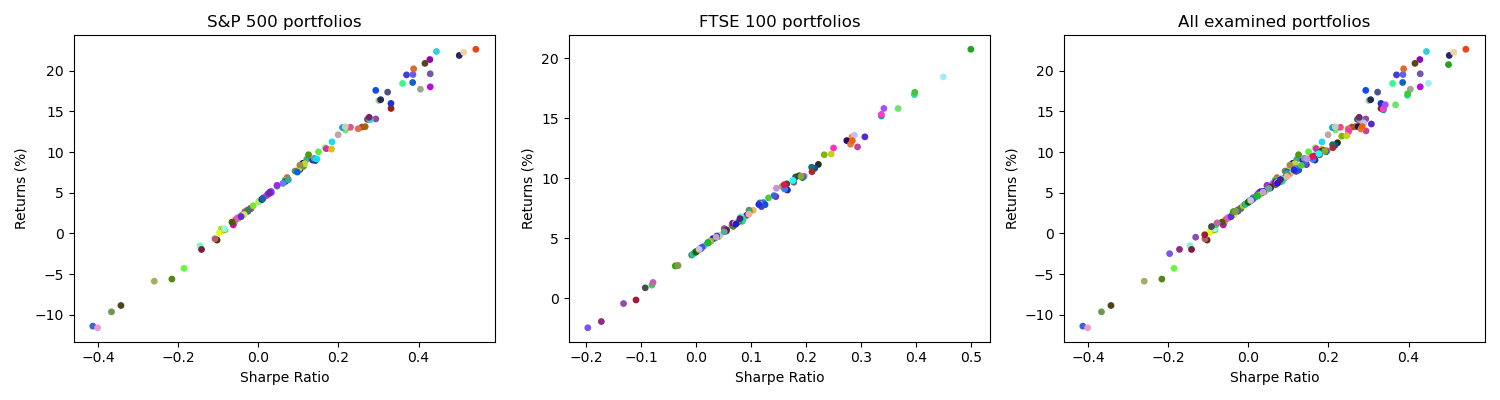
\includegraphics[width=\textwidth]{images/returns.png}
  \caption{Returns}
  \label{fig:returns}
\end{figure*}

The 108 portfolio-building strategies were tested across two non-overlapping subsets of the global financial markets: the S\&P 500 index and the FTSE 100 index.
Fig.~\ref{fig:returns} summarizes the returns obtained when applying our method to select stocks from each index, ordered by Sharpe ratio.
The Sharpe ratio compares a portfolio’s returns with its associated risk, indicating how much of the return can be attributed to excess volatility.
Generally speaking, the higher the ratio the better.

% TODO: Falar sobre qual e o melhore no S&P, FTSE e quais sao os 3 melhores globais.

% TODO: Mostrar grafo das comunidades para os 3 melhores.
% TODO: Discutir uma beca os grafos

%TODO: Atualizar a imagem depois
\begin{figure*}[b]
  \centering
  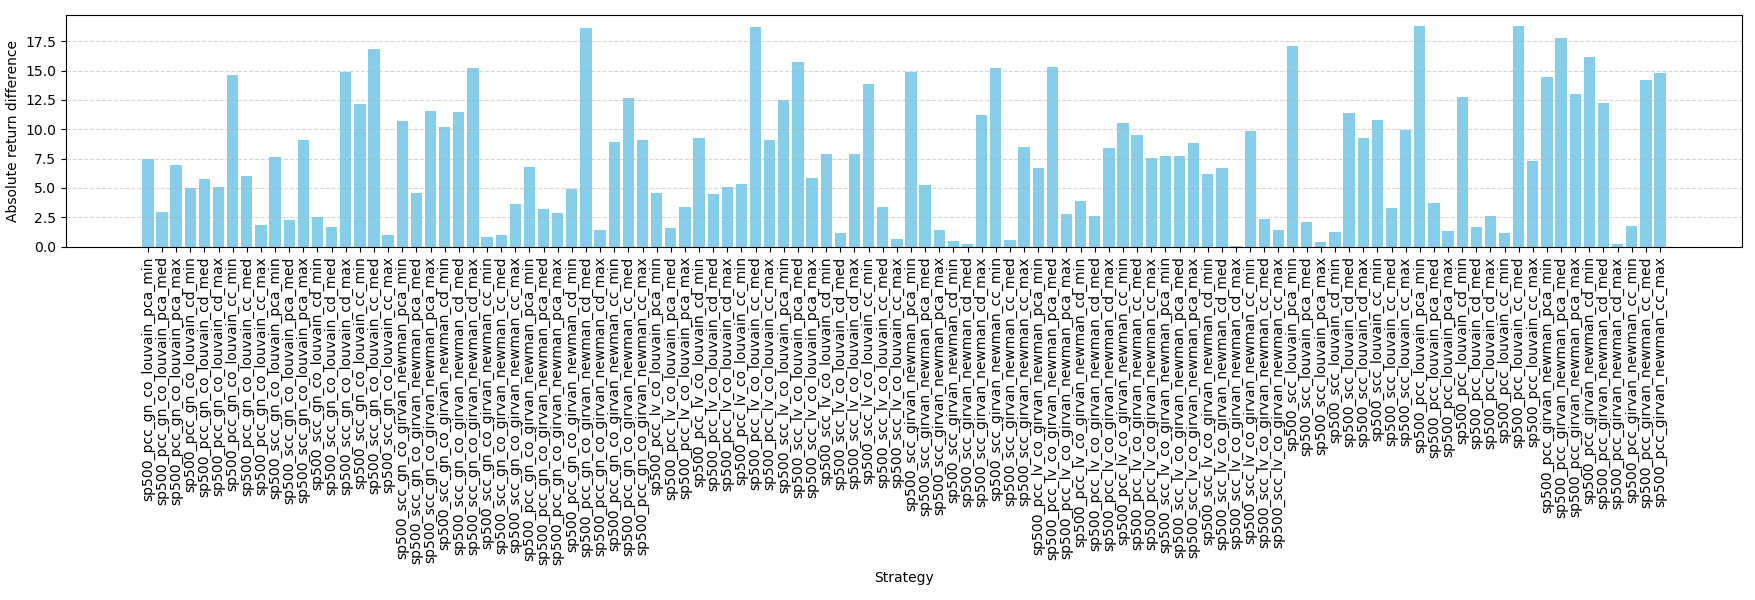
\includegraphics[width=\textwidth]{images/differences.png}
  \caption{Returns}
  \label{fig:returns}
\end{figure*}

% TODO: Falar sobre quais são os 3 com diferencas menores e os 3 com diferencas maiores, dizer o ranking em que estao em termos de returns para os dois indices.
% TODO: Discutir que os 3 com diferencas menores sao, em principio, estrategias mais robustas e que dependem menos de carateristicas especificas de um mercado em particular.

\section{Discussion \& Conclusion} \label{conclusion}

% Falar das diferencas em resultados do nosso para o deles.
% -> Fizeram no Covid que é um periodo especialmente pouco representativo, portanto faz sentido que as suas estrategias generalizem mal para outros periodos.
% -> Estas estrategies nao conseguem capturar todas as intricasies presentes nos mercados financeiros, é dificil arranjar um metodo que generalize bem para varios mercados e periodos diferentes.
TODO

%%
%% The next two lines define the bibliography style to be used, and
%% the bibliography file.
\bibliographystyle{ACM-Reference-Format}
\bibliography{references.bib}

\newpage

\end{document}
